\chapter{Løsning}

\section{\textbf{Om løsningen}}
\newthought{Middagsassistenten er en videreutvikling} av den eksisterende mobilapplikasjonen til Kolonial.no. Løsningen vi har laget er en separat applikasjon, men skal fungere som en implementasjon og videreutvikling i den eksisterende løsningen.

\section{\textbf{Plattform}}
\newthought{Vi valgte i utgangspunktet} å lage en Android-applikasjon i Java. Vi ønsket å nå en mindre målgruppe for å ha mer kontroll over tilbakemeldingene som vi fikk for endringene, så vi hyppig kunne levere nye endringer eller rulle de tilbake. Etter jul gikk vi bort i fra Android til fordel for Ionic, et rammeverk for kryssplattformutvikling som gir støtte for både iOS og Android. Fordelen med å bytte til Ionic er at vi kunne utnytte ressursene i teamet bedre, siden flere kunne bidra med HTML/CSS. I tillegg gjør Ionic det mulig å levere en løsning for flere plattformer med kun én kodebase. Vi har valgt å ikke gi støtte for Windows Phone siden brukermassen er såpass liten, og designendringer ville bundet opp mye ressurser i teamet.

\section{\textbf{Database}}
\newthought{Vi bestemte at vi skulle} bruke Parse som backend for database i starten av prosjektet, men da vi byttet fra Android til kryssplattform, endret vi også løsning for databasen. Vi har valgt å bruke Firebase, av flere grunner. Blant annet er både Parse og Firebase flate databaser som bygger på NoSQL, som gjør at overgangen er liten. NoSQL er en type database som ikke har relasjoner mellom data som er lagret. Dette gir oss da full frihet på å strukturere data slik vi vil, uten å måtte tenke på hvordan de henger sammen med hverandre. I tillegg, og kanskje den viktigste grunnen er at siden Ionic er basert på Angular, har rammeverket <<out-of-box>>-støtte for Firebase som gjør at det er lett å ta i bruk. Vi beskriver strukturen på databasen senere i dokumentet.

\section{\textbf{Kolonial.no sitt API}}
\newthought{Vi har valgt} å bruke Kolonial.no sitt API i den grad det har vært mulig. API er et programmeringsgrensesnitt som lar oss aktivere deler av en programvare fra en annen program. Denne delen blir aktivert ved hjelp av en endpoint, som er en modul som blir utsatt i dette grensesnittet. Dette gjorde at vi hadde tilgang til deres egne produkter, produktinformasjon, søkefunksjonalitet m.m. ved hjelp av endpoints Kolonial.no har definert. I tillegg vil det gjøre det lettere for Kolonial.no å implementere vår løsning i sin egen eksisterende app. Som en effekt av at vi tok i bruk API-et deres har vi sluppet å lagre mye informasjon i egen database.

\section{\textbf{Beskrivelse av løsningen}}
\newthought{Vi vil her} gå gjennom den tekniske løsningen.
Det vil vises en figur som viser den aktuelle siden, og paragrafer som beskriver siden funksjonelt og visuelt.

\subsection{\textbf{Overordnet om det visuelle}}
Appen er en utvidelse av Kolonial.no sin eksisterende app og vi har derfor valgt å fortsette med Kolonial.no sitt tema/layout for å holde et konsistent design gjennom hele løsningen (\url{http://brand.kolonial.no/d/EnPDNkuST9re/merkevare#/elementer/farger}). Vi har også utviklet vårt eget basert på Kolonial.no sine farger og former, hvor vi har egne sider og unikt innhold. 

Vi har utover dette fulgt retningslinjer om universell utforming ved å ha sterke kontrastfarger, og bruke farger som fungerer for fargeblinde. Mer om det visuelle vil stå som eget punkt under beskrivelse av sidene. Når vi beskriver det visuelle vil vi ta utgangspunkt i fargepaletten og benytte fargenavn.

\begin{figure}[H]
    \includegraphics[width=\textwidth]{figures/teknisk/farger}
    \caption[Fargepalett]{Fargepalett
    \label{fig:color_palette}}
\end{figure}

Kolonial.no har et lite antall knapper med oransje/gul bakgrunn og hvit skrift. For å holde designet konsistent med resten har vi valgt å beholde dem, selv om oppfatningen vår egentlig er at disse har dårlig kontrast og dermed synlighet - da spesielt for svaksynte. Vi har sett på muligheten for å skyggelegge dem, men knappene er av liten størrelse og de har en kant på teksten, og dette kan for noen gjøre at teksten er mindre synlig. Hvis teksten hadde vært større ville vi ha løst problemet med skyggelegging eller kant, som vist i eksempelet under.

\begin{figure}[H]
    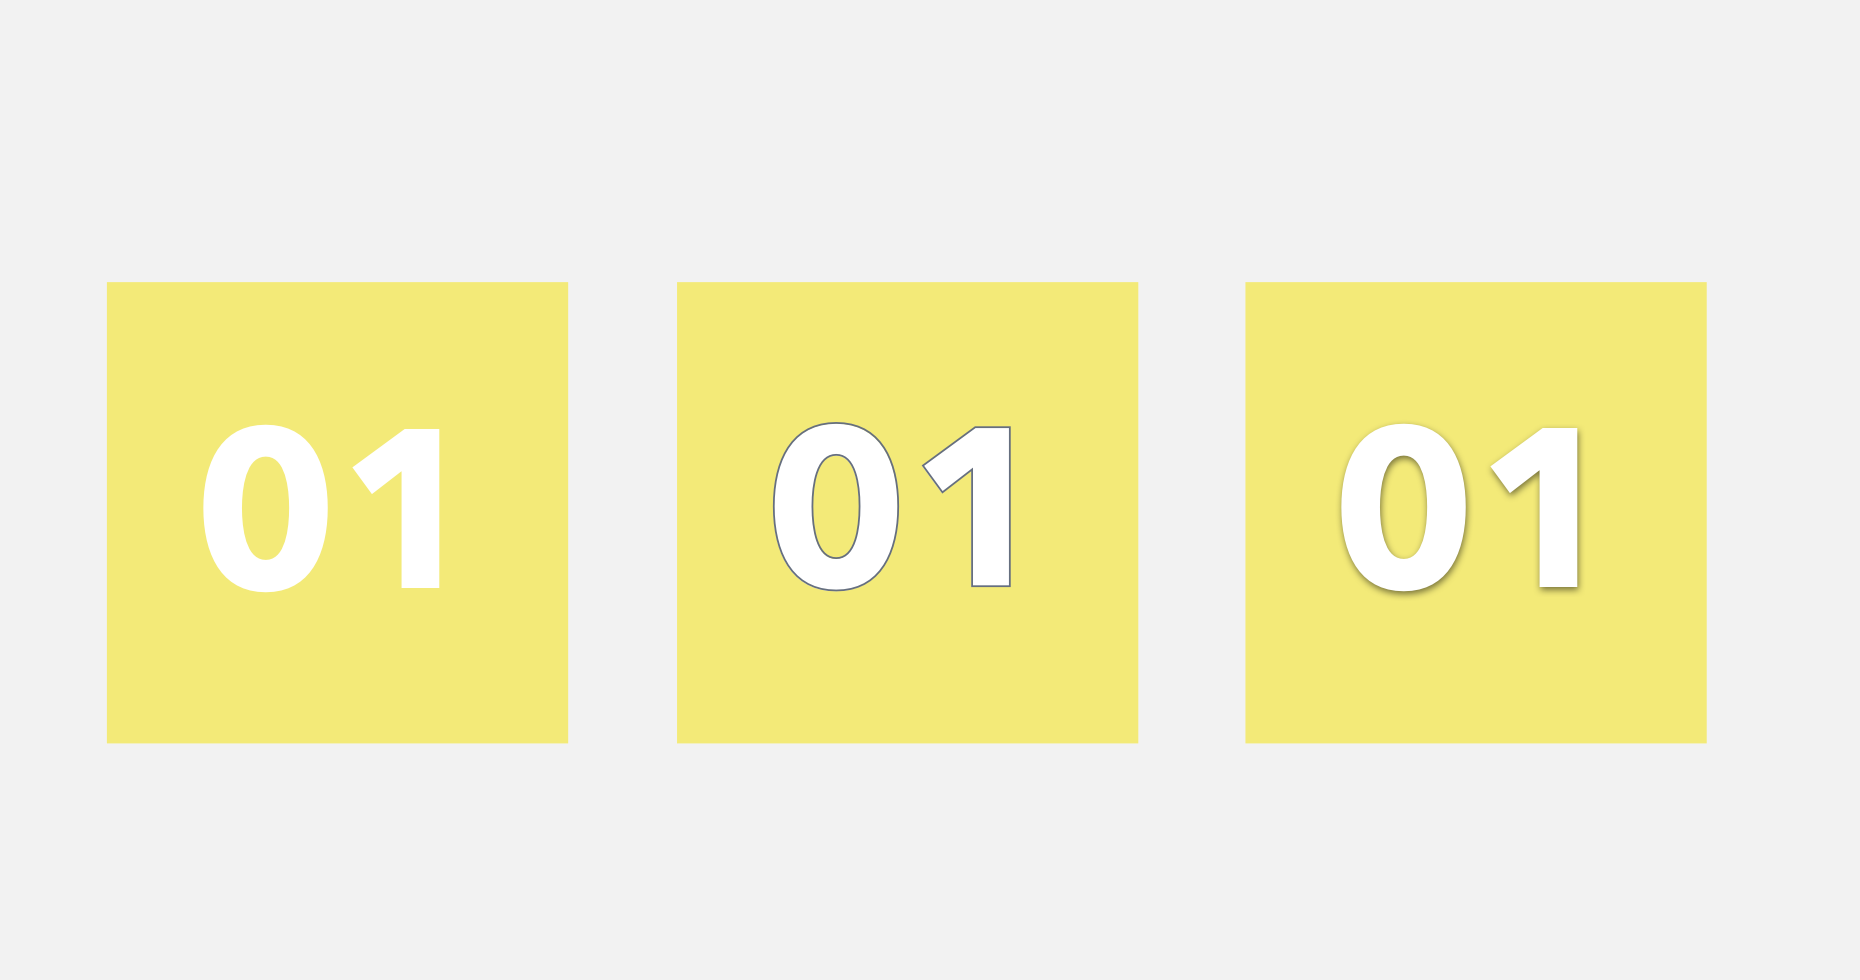
\includegraphics[width=\textwidth]{figures/something}
    \caption[Fargekontrast]{Eksempel på tiltak til hvordan synliggjøre hvit tekst på gul/oransje bakgrunn
    \label{fig:color_contrast}}
\end{figure}

Selve layouten har vi forholdt oss til en utforming som er godt kjent for de fleste med et konsistent design hvor vi følger normen for hvordan apper ser ut i dag og hvordan verktøyene allerede har predefinerte maler for hvordan layoutet skal se ut. For eksempel er hovedmenyen i bunn og hamburgermeny på topp. Vi har forholdt oss til hvordan appen til Kolonial ser ut i dag, men har byttet ut noen valg for å få tilpasset appen til å passe inn med vårt konsept.

Tilbakemeldinger til brukeren på utførte handlinger kommer ofte i en “Toast”. Denne dukker opp som en boks nederst på siden og er slik som det er på veldig mange apper. Vi skulle ønske at noen av disse kom bedre innenfor synsfeltet hvor brukeren har oppmerksomheten, men siden dette er en standard, og den har farger og bevegelser så har vi ikke gjort noe med dette. Det ville også føre til betydelig ekstraarbeid som vi ikke ville ha hatt tid til i disse iterasjonene.

%%%%%%%%%%%%%%%%%%%%%%%% LOGIN %%%%%%%%%%%%%%%%%%%%%%%% 
\subsection{\textbf{Innlogging}}
\begin{figure}[H]
    \includegraphics[width=\textwidth]{figures/teknisk/login/login}
    \caption[Innlogging 1]{Innloggingsside
    \label{fig:login}}
\end{figure}

\subsubsection{\textbf{Funksjonelt}}
Innloggingssiden brukes for å enten logge inn i appen, eller for å registrere seg. For å logge inn må brukeren ha en eksisterende konto hos Kolonial.no. Hvis brukeren ikke har det, så kan en ny bruker registreres ved å trykke på <<... Registrer deg her!>>. Grunnet mangel på endpoint for registrering hos Kolonial.no blir brukeren videresendt til deres egen registreringsside i en intern nettleser. 

Når bruker logger inn med sin påloggingsinformasjon fra Kolonial.no, sendes det en forespørsel til vår Firebase database for å se om vi har en lokal kopi av brukeren. Hvis vi ikke har en kopi av brukeren, så blir det opprettet en forespørsel til Kolonial.no sitt API for å autentisere bruker og få tilbake noe data om brukeren. Informasjonen vi får tilbake blir lagret i en Firebase kolleksjon. Neste gang bruker logger inn, så eksisterer det en lokal kopi i vår database og vi slipper å gjøre en forespørsel mot Kolonial.no sitt API. Vi mellomlagrer brukerdata for å kunne lagre favorittoppskrifter og beholdning til brukeren. Vi har ikke tatt hensyn til personvernforordningen GDPR (General Data Protection Regulation) siden appen skal fungere som en videreutvikling av deres eksisterende løsning. Vi forutsetter derfor at Kolonial.no følger de nye personvernsreglene.

\begin{figure}[H]
    \includegraphics[width=\textwidth]{figures/teknisk/login/users}
    \caption[Innlogging 2]{Dette er hvordan brukerinformasjon lagres hos oss. Vi lagrer det som returneres av API-et.
    \label{fig:userdb}}
\end{figure}

\subsubsection{\textbf{Visuelt}}
På siden for innlogging hadde vi opprinnelig en oransje farge som bakgrunnsfarge på prototypene. Vi valgte denne da dette var en farge vi hadde sett i Kolonial.nos opprinnelige løsning, og vi tenkte at konsistent design var å foretrekke. Dette gjorde vi selv om vi var under oppfatningen av at det strider med prinsipp for universell utforming, kontrast, og fargebruk. Oransje med hvit tekst gir ikke ideell synlighet. Dette endret vi på etter vi hadde hatt veiledning med produkteier. Vi endret til mer nøytrale og stilrene farger. Vi gikk for en grønnfarge vi tidligere hadde sett i Kolonial.nos løsning. 

Før du logger inn og trykker på feltene er feltene hvite med en grå understrek. Når du har fylt ut en gyldig epostadresse blir streken grønn samtidig som streken til feltet for passord blir oransje for å hinte til neste steg for brukeren. Ved feil inntasting blir streken rød under det feltet det gjelder. Vi har brukt farger som fungerer for de fleste, selv om man er fargeblind.

Knappen for å logge inn er satt filter på for å få ned kontrasten slik at når brukernavn og passord er fylt ut så blir knappen tydeliggjort med sterk kontrast, og viser at du er klar til å logge inn. Dette hjelper brukeren til å ikke gjøre feil, forstå og få tilbakemelding hva som skjer og hva brukeren har gjort.


%%%%%%%%%%%%%%%%%%%%%%%% HJEM %%%%%%%%%%%%%%%%%%%%%%%% 
\subsection{\textbf{Hjem og strekkodeleser}}
\begin{figure}[H]
    \includegraphics[width=\textwidth]{figures/teknisk/login/hjem}
    \caption[Hjem]{Hjemside [t.v] og strekkodeleser [t.h]
    \label{fig:hjem}}
\end{figure}

\subsubsection{\textbf{Funksjonelt}}
Hjemsiden er statisk og bare en visuell representasjon av deres eksisterende løsning.
I toppmenyen, øverst til venstre har vi strekkodeleser slik at man raskt og lett kan finne et produkt. Øverst til høyre har vi en hamburgermeny for å få aksessert brukerinnstillinger og logg ut-knapp.

\subsubsection{\textbf{Visuelt}}
Forsiden er bare et eksempel på layout, og ikke lagt mye vekt på da dagens kolonial.nos hjemmeside skal brukes ved en implementering. Med tanke på at oppskrifter er en stor del av vår idé så har vi valgt å ta med det på forsiden, som en ukemeny.

\subsection{\textbf{Strekkodeleser}}
\subsubsection{\textbf{Funksjonelt}}
Når man klikker seg inn på barcode scanneren øverst i venstre hjørne på hjem siden, kommer opp bilde 1. Her plasserer man bare strekkoden slik at den er på linje med den røde linjen på kameraet. Når man har scannet varen kommer man rett inn på produktsiden for produktet. 

En av plussidene med at vi byttet til Ionic er at vi har tilgang til et større bibliotek med moduler. Strekkodeleser er en modul som allerede eksisterer for Cordova, noe som betydde at vi slapp å implementere dette selv og dermed sparte mye tid på det. Cordova er mellomlaget mellom Ionic og telefonen, som lar oss ta i bruk funksjoner vi ellers ikke hadde hatt tilgang til (eks: kamera). Når bruker trykker på strekkoden på bilde 1, så blir det sendt en forespørsel til denne modulen som da starter opp kamera. Når en strekkode har blitt lest, så blir verdien på strekkoden returnert tilbake. Denne verdien bruker vi for å gjøre et søk i produktdatabasen til Kolonial.no, ved hjelp av deres API. Hvis produktet finnes i databasen deres, blir brukeren sendt videre til produktet. Hvis produktet ikke finnes, får bruker en melding om at dette er en vare som ikke er tilgjengelig.

\subsection{\textbf{Visuelt}}
På figuren ~\ref{fig:hjem} til høyre har vi strekkodeleser. Vi har prøvd å lage et ikon som passer overrens med resten av utforming på siden, samtidig som vi ønsker at brukeren skal gjenkjenne ikonet. Se produktside (\ref{sec:produkt}) for mer.

%%%%%%%%%%%%%%%%%%%%%%%% SØK %%%%%%%%%%%%%%%%%%%%%%%% 
\subsection{\textbf{Søk}}
\begin{figure}[H]
    \includegraphics[width=\textwidth]{figures/teknisk/sok/sok}
    \caption[Søkside]{Søkside
    \label{fig:sok}}
\end{figure}

\subsubsection{\textbf{Funksjonelt}}
Siden lar bruker søke gjennom varer i produktdatabasen til Kolonial.no. 
For hver endring i søkelinjen, blir det gjort en forespørsel mot Kolonial.no sitt API som returnerer en liste over produktene den finner med gitte søkekriterier. Vi begrenser antall resultater til 15, for å ta hensyn til databruk. Disse resultatene vil så bli presentert til brukeren (se figur \ref{fig:sok}).

\subsubsection{\textbf{Visuelt}}
Her har vi valgt å bruke sterke kontraster, ved å ha <<mørk>> som tekstfarge, mot hvit bakgrunn, samt utheve produktnavnet, og minske prisen. Da får vi størst blikkfang på produktbilde- og navn. 

%%%%%%%%%%%%%%%%%%%%%%%% PRODUKT %%%%%%%%%%%%%%%%%%%%%%%% 
\subsection{\textbf{Produkt}}
\label{sec:produkt}
\begin{figure}[H]
    \includegraphics[width=\textwidth]{figures/teknisk/produkt/produkt}
    \caption[Produkt]{Produktside
    \label{fig:produkt}}
\end{figure}

\textbf{Funksjonelt:}
Her kan du flytte produktet mellom kategorier i din beholdning, ved å klikke på - og +. Når bruker har gjort endringene sine og navigerer ut av siden, blir det gjort en forespørsel mot Firebase databasen om å lagre endringene bruker har gjort. Mer om hvordan databasen for total i beholdning og enkeltkategorier er satt opp kan leses om i \ref{sec:beholdning}

\textbf{Visuelt:}
Vi støtter på en logisk brist i visning av varer. Vi kom fram til at vi hadde tre forskjellige visninger av varer:\newline
1. Når man scanner en vare.\newline
2. Når man skal se på varen.\newline
3. Når man skal flytte og kjøpe varen.\newline 

Dette så vi først når vi begynte å bygge applikasjonen, selv etter tre prototyper og brukertesting.

Grunnen til at vi ikke så denne logiske bristen kan ha hatt en sammenheng med at vi har tenkt at Kolonial.no allerede har disse løsningene og at vi dermed ikke trengte å tenke på det. Vi ble klar over at vi ikke kunne vise en vare uten at kjøpknappen er til stede.

Med bakgrunn i dette tok vi en runde på tavlen og fikk tegnet opp alle varianter av mulige visninger av en vare og hvordan man navigerer dit. Med denne prosessen så vi at dette kunne være en visning som kunne være overalt uavhengig om man går inn på en vare i beholdning eller scanner en vare. 

Dette gir fordeler for brukeren ved at de kun trenger å forholde seg til en type side. 

Vi så fort at det kom til å bli mye informasjon på visningen av en vare og måtte kutte eller sørge for at bruker ikke ble presentert med all informasjon om en vare på en gang. Løsningen vi kom frem til var en liste med informasjon om varen og beholdning.

%%%%%%%%%%%%%%%%%%%%%%%% OPPSKRIFTER %%%%%%%%%%%%%%%%%%%%%%%% 
\subsection{\textbf{Oppskrifter}}
\begin{figure}[H]
    \includegraphics[width=\textwidth]{figures/teknisk/oppskrifter/oppskrifter}
    \caption[Oppskrifter]{Oppskrifterside
    \label{fig:oppskrifter}}
\end{figure}

\subsubsection{\textbf{Funksjonelt}}
Oppskrift siden er bygd opp slik at man kan få forslag til hva man skal ha til middag. Øverst har man fire forskjellige kategorier man kan velge mellom.

\textbf{Populære:}
\\Inne på denne kategorien ligger de oppskriftene som har fått flest favoritter fra brukere. Hvor populær en vare er blir sporet ved å ha ett <<integer>-felt i oppskriften, som økes og reduseres når en bruker legger til eller fjerner oppskriften fra sine favoritter.

\textbf{Favoritter:}
\\Når man er inne på en oppskrift har man mulighet til å legge oppskriften inn i favoritter, som best passer din beholdning, og legges da inn her. Hvilke oppskrifter en bruker har favorisert blir lagret i en kolleksjon <<favorites>>, som er en subkolleksjon av bruker-dokumentet (se figur \ref{fig:userdb}).

\textbf{Dine varer:}
\\Dine varer er basert på varene man har lagt inn i sin beholdning. Øverst i venstre hjørnet står det hvor stor andel av varene man har i beholdningen. Dette tallet regnes ut ved å sammenligne varene som bruker har i beholdning, med varer som oppskriften trenger. Basisvarer blir ikke tatt med når match blir regnet ut.

\textbf{Pris:}
\\Er sortert etter hvilke retter som er billigst. Pris blir regnet ut ved å ta i betraktning hva bruker allerede har, slik at kun varene bruker mangler blir summert i pris.

\begin{figure}[!h]
    \includegraphics[width=\textwidth]{figures/teknisk/oppskrifter/oppskrifterdb}
    \caption[Oppskrifter - Databasestruktur]{Databasestruktur for oppskrifter
    \label{fig:oppskrifterdb}}
\end{figure}

\newpage
\textbf{Visuelt:}
Denne siden finnes allerede hos Kolonial.no. På den eksisterende er det to oppskrifter i bredden, mens vi har valgt å ha én oppskrift i bredden. Dette for å ha fokus på én oppskrift av gangen. Dette gir større plass til bilde slik at brukeren skal se retten/oppskriften bedre og bli fristet. Vi har også lagt til en knapp for å gjøre det mer intuitivt å klikke på oppskriften.

På bildet av oppskrifter basert på beholdning har vi en visuell fremstilling av hvor stor prosentdel av oppskriften bruker har i beholdning. I prototypen kan denne bytte farge med andelen av prosentsats. Dette vil si at om man har alle ingrediensene til en oppskrift, eller mer, så er dette feltet grønt med 100 \%.

Vi har brukt <<primær>> som farge for en aktiv kategori og knapp for å
skape blikkfang. I tillegg bruker vi <<mørk>> som farge på tekst mot hvit bakgrunn
for å ta hensyn til universell utforming.


%%%%%%%%%%%%%%%%%%%%%%%% ENKELTOPPSKRIFT %%%%%%%%%%%%%%%%%%%%%%%% 
\subsection{\textbf{Enkeltoppskrift}}
\begin{figure}[H]
    \includegraphics[width=\textwidth]{figures/teknisk/oppskrifter/oppskrift}
    \caption[Oppskrift]{Side for oppskrift
    \label{fig:oppskrift}}
\end{figure}

\textbf{Funksjonelt:}
I oppskriften ser man en liste over ingredienser, og hvor mange man trenger av hver. Her kan man justere porsjoner med pluss- og minus-tegnene. Når man legger til og trekker fra porsjoner endres også volumet av ingrediensene man trenger. Dersom varen er en basisvare, som f.eks. krydder eller vann vil det stå <<BASIS>> fremfor mengde. Dersom man likevel trenger basisvaren kan man trykke seg inn til produktsiden og kjøpe derifra. I en ferdig løsning ville vi hentet ut oppskrifter fra API-et deres, men grunnet vår ekstrafunksjonalitet som <<Oppskrifter basert på beholdning>> får vi ikke ut all informasjon vi trenger. Vi har derfor valgt å lage noen <<dummy>>-oppskrifter for å vise hvordan det ville fungert i en vanlig løsning.

\subsubsection{\textbf{Bruk Oppskrift:}}
Denne knappen vil trekke fra alle varene som brukes i oppskrifter fra beholdningen din, og regne ut riktig mengde. Dette gjør det mulig å bruke f.eks. 1/3 av en hel ost fremfor at hele produktet fjernes fra beholdning. 

\subsubsection{\textbf{Kjøp: }}
Vi har kuttet hele kjøpsprosessen ettersom den allerede finnes i den eksisterende løsningen. Vi valgte å gjøre det slik at produktene du <<kjøper>>, automatisk blir lagt til usortert i beholdningen.

\subsubsection{\textbf{Favoritt: }}
Øverst i høyre hjørne finner du et hjerteikon som tillatter brukeren å favorisere en oppskrift. Dette vil øke oppskriftens rangering i <<Populære>>-kategorien, samt legge oppskrifter til i <<Favoritter>>-kategorien.

\newpage
\textbf{Visuelt:}
Fargevalgene vi endte opp med var:\newline
<<pris>>: Grå bakgrunn på basisvarer for å ikke ta unødig stor oppmerksomhet.\newline
<<bringebær>>: Dersom brukeren mangler varer ville det være uthevet i en rødfarge for å skape kontrast og få stor oppmerksomhet.\newline
<<grønn>>: Tilsvarende bringebær brukes grønnfargen for å fange oppmerksomhet, og grønn oppleves som en farge for at noe er <<riktig>>. Det representerer at brukeren har nok av en vare.

%%%%%%%%%%%%%%%%%%%%%%%% BEHOLDNING %%%%%%%%%%%%%%%%%%%%%%%% 
\subsection{\textbf{Beholdning}}\label{sec:beholdning}
\begin{figure}[H]
    \includegraphics[width=\textwidth]{figures/teknisk/beholdning/beholdning}
    \caption[Beholdning]{Beholdningsside
    \label{fig:beholdning}}
\end{figure}

\textbf{Funksjonelt:}
På beholdningssiden ser man alle varene man har lagt til i beholdning. Dersom man ikke
manuelt sorterer varer vil det legges til i usortert. Man kan velge hvor mange av en vare man har, og det vil slettes automatisk dersom antallet er 0.

\begin{figure}[H]
    \includegraphics[width=\textwidth]{figures/teknisk/beholdning/beholdningdb}
    \caption[Beholdning - Database]{Referansen til en kategori i databasen ser slik ut: storage/{brukerId}/{kategoriId}.
Tallene 0-4 i kolleksjonen referer til en spesifikk kategori. Innenfor kategorien blir produktet lagret med produkt id som dokument id. Kolleksjonen quantity inneholder et dokument med produkt id som dokument id, og dette dokumentet har et felt ‘total’ som holder telling på totalsummen av produktet brukeren har.
    \label{fig:beholdningdb}}
\end{figure}

\textbf{Visuelt:}
Øverst har vi et søkefelt for å fort finne ønsket produkt.
Under har vi kategorier for å lettere ha oversikt over hvor diverse produkter befinner seg. Så blir produktene brukeren har i beholdningen listet nedover med oversikt over hvor mye av produktet du har igjen.

%%%%%%%%%%%%%%%%%%%% DESCRIPTION %%%%%%%%%%%%%%%%%
\section{\textbf{Installasjon av løsning}}
\subsection{\textbf{Brukerinformasjon}}
1. Brukernavn: gruppe16smidig@gmail.com\\
2. Passord   : Kolonial123\\
$\rightarrow$ Eventuelt egen bruker hos Kolonial.no

\subsection{\textbf{Google Play Store}}
Løsningen er tilgjenglig på Google Play Store for Android-enheter.
\url{https://play.google.com/store/apps/details?id=no.octopod.smidig.kolonial}

\subsection{\textbf{Forkrav for bygging av prosjekt}}
Det forutsettes at Cordova, Ionic og Node er installert for å kunne bygge løsningen selv.

\subsubsection{\textbf{Installering av forkrav}}
\paragraph{\textbf{Node}}
\subparagraph{Windows}
Node for Windows kan lastes ned fra \url{https://nodejs.org/en/download/}.

\subparagraph{MacOS}
Installer Node med cURL:
\begin{minted}[breaklines]{bash}
curl "https://nodejs.org/dist/latest/node-${VERSION:-$(wget -qO- https://nodejs.org/dist/latest/ | sed -nE 's|.>node-(.).pkg.*|\1|p')}.pkg" > "$HOME/Downloads/node-latest.pkg" && sudo installer -store -pkg "$HOME/Downloads/node-latest.pkg" -target "/"
\end{minted}

\subparagraph{Linux}
\begin{minted}[breaklines]{bash}
curl -sL https://deb.nodesource.com/setup_8.x | sudo -E bash - sudo apt-get install -y nodejs
\end{minted}

\paragraph{\textbf{Ionic og Cordova}}
\paragraph{Windows, MacOS og Linux\newline}
Kjør følgende kommando i terminalvinduet:
\begin{minted}[breaklines]{bash}
npm install -g ionic cordova
\end{minted}

\subsection{\textbf{Kjøre løsningen}}
Kildekoden for løsningen kan lastes ned fra \url{https://github.com/Westerdals/PRO200-17-16/archive/master.zip}.

\subsubsection{\textbf{Kjør på Android}}
Android SDK og Java JDK er forkrav for å kunne bygge APK for Android.
Android SDK kan lastes ned fra \url{https://developer.android.com/studio/}.
Java JDK kan lastes ned fra \url{http://www.oracle.com/technetwork/java/javase/downloads}.

Koble til telefonen og kjør følgende kommando i rotmappen til løsningen:
\begin{minted}[breaklines]{bash}
ionic cordova run android
\end{minted}

\textit{Løsningen kan også kjøres i Android Emulator ved å kjøre samme kommando uten å koble til telefon.}

\subsubsection{\textbf{Emulering i nettleser}}
\textit{Å kjøre løsningen i web er ikke anbefalt. Applikasjonen fungerer ikke som tiltenkt, grunnet CORS-restriksjoner i Kolonials API}.

Kjør følgende kommando i rotmappen til løsningen:
\begin{minted}[breaklines]{bash}
ionic serve --lab
\end{minted}
\textbf{NB! CORS må skrus av for å kunne kjøre løsningen i nettleser!}

\paragraph{\textbf{Deaktiver CORS i Google Chrome}}\mbox{}
\subparagraph{{Windows}}\mbox{}\\
1. Lukk alle Chrome-vinduer\\
2. Kjør følgende kommando i mappen chrome er installert i:
\begin{minted}[breaklines]{bash}
chrome.exe --disable-web-security --user-data-dir
\end{minted}

\subparagraph{{MacOS}}\mbox{}\\
1. Lukk alle Chrome-vinduer\\
2. Kjør følgende kommando i terminalvindu:
\begin{minted}[breaklines]{bash}
open -a Google\ Chrome --args --disable-web-security --user-data-dir
\end{minted}

\subparagraph{{Linux}}\mbox{}\\
1. Lukk alle Chrome-vinduer\\
2. Kjør følgende kommando i terminalvindu:
\begin{minted}[breaklines]{bash}
google-chrome --disable-web-security --user-data-dir
\end{minted}

\paragraph{\textbf{Deaktiver CORS i Safari}}\mbox{}\\
1. Aktiver Developer Tools in Safari\\
2. Develop $\rightarrow$ Disable Cross-Origin Restrictions

